\documentclass{article}
\usepackage{natbib}
\usepackage{amsmath}
\usepackage[small]{caption}
\usepackage{wrapfig}
\usepackage{graphicx}
\usepackage{placeins}
\usepackage[top=1in, bottom=1in, left=1.25in, right=1.25in]{geometry}
\begin{document}
\title{Research Statement: Understanding pulsars \& neutron stars, for and with gravitational wave detections}
\author{Shu-Xu Yi}
\date{\today}
\maketitle
My research interests focus on three strongly related fields: pulsar timing, gravitational wave astronomy \& electromagnetic wave radiation mechanism of neutron star binaries. 

Pulsar is one class of end points of massive stars' evolution, which is a rapidly spinning, highly magnetized neutron star (or quack star). Their extremely stable and regular spin, together with their lighthouse-like, collimated radiation beams, makes them ideal test fields of physics laws in extreme conditions, and possible to explore the nature of neutron stars/neutron star binaries. Pulsar can also play the role as galaxy-scale gravitational wave detector, aiming at nanohertz gravitational wave, among sources of which there are massive black hole binaries in merged galaxies. Besides, the neutron star binaries are important gravitational wave sources themselves, which can be studied with ground-based gravitational wave observatories, e.g., LIGO. 
\hspace*{- 4 cm}
\begin{figure}[h!]
\centering
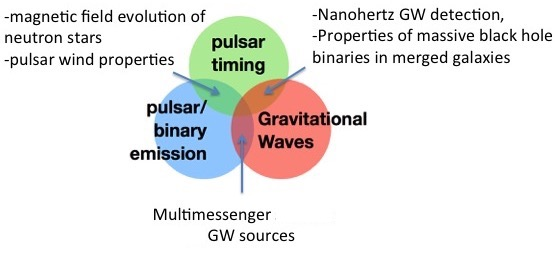
\includegraphics[width =9cm, trim=0 0 2.9cm 0cm]{research_interest_complex.jpg}
\caption{Fields which I am interested in}
\end{figure}
\section{Pulsar timing}
Pulsars rotate at extremely stable rate, therefore signals from a pulsar arrival at a telescope in the time interval that changes tiny over a long time. Since a pulsar is a spinning magnetic dipole, there is a constant spin frequency down rate due to the magnetic dipole radiation.  

Many factors can give rise to additional period changes beyond the constant spin frequency derivative. In other words, studying the spin period evolution can give clues to many questions in astrophysics. The applications of pulsar timing is the topic of my Ph.D thesis, supervised by Prof. Zhang Shuang-Nan. One major application is to use a pulsar/an array of pulsars as a detector of gravitational wave transpassing the space between a pulsar/pulsars and Earth. We used the timing data of PSR B1937+21 from Jodrell Bank telescope and WSRT telescope, to constrain the strain of individual nanohertz gravitational wave \citep{2014MNRAS.445.1245Y}. The main collaborator of this project is Prof. Ben Stappers, who is an expert on pulsar timing from Jodrell Bank Observatory. Other applications include studying the magnetic field evolution of neutron stars \citep{2015MNRAS.454.3674Y}. 

\section{Radiation mechanisms of neutron star binaries}
After obtained the Ph.D degree, I have been in the group of Prof. K.S. Cheng as a postdoctoral fellow. Prof. Cheng is renowned for his study on neutron stars emission mechanism. We started projects on modeling the Gamma-ray emission mechanism of neutron star-binaries \citep{2017ApJ...844..114Y, 2017arXiv170708263Y}. My experience on pulsar timing brought us new perspectives. I proposed an independent way using pulsar timing to study the properties of pulsar wind in a double pulsar system \citep{c}. We are currently working on a project constraining the mass transfer process between a gamma-ray pulsar binary with timing data. 

Among neutron star binaries, there are neutron star-black hole binaries, neutron star-pulsar binaries and double pulsars. Those are important sources of gravitational wave for ground-based detectors. 

\hspace*{- 4 cm}
\begin{figure}[t]
\centering
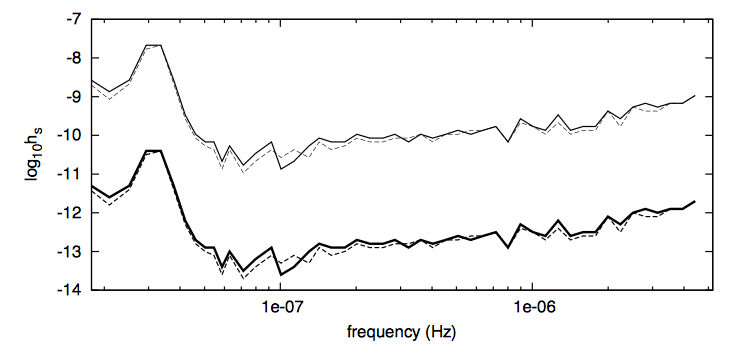
\includegraphics[width =9cm, trim=0 0 2.9cm 0cm]{GWlimit.png}
\caption{The upper limit of individual gravitational wave sources, set with timing of PSR B1937+21. See details in \citep{2014MNRAS.445.1245Y}.}
\end{figure}
\hspace*{- 4 cm}

\begin{figure}[b!]
\centering
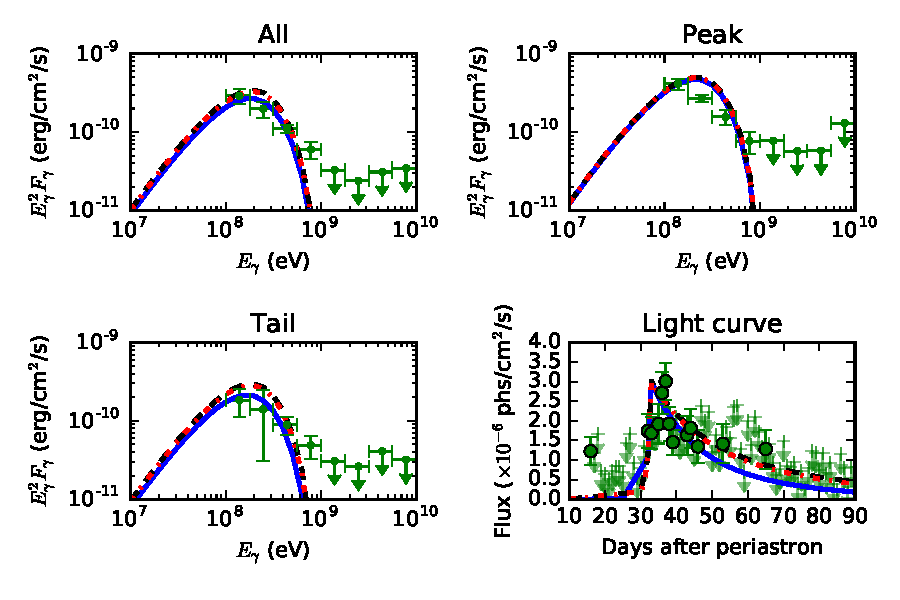
\includegraphics[width =0.83\textwidth, trim=0 0 0cm 0cm]{FourForOne.pdf}
\caption{Modeling the SEDs and light curve of gamma-ray binary PSR B1259-63/LS2883. See \cite{2017ApJ...844..114Y} for details.}
\end{figure}
\newpage
\section{Gravitational wave astronomy}
I am interested in gravitational wave astronomy for a long time. Except for the work mentioned above, we proposed an algorithm that extends the frequency range of gravitational wave detectable with pulsar timing \citep{2016SCPMA..59h..95Y}. I also explored the potential effect of the gravitational wave Cherenkov radiation on cosmology \citep{2017MPLA...3250059Y}. I hope to enrich my experience on gravitational wave detection, especially on ground-based gravitational wave detection in the further. I am particularly interested in studying neutron star binaries as sources of gravitational wave. 
\begin{figure}[h!]
\centering
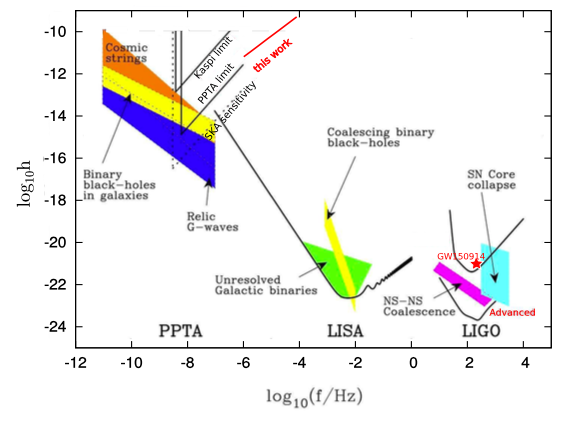
\includegraphics[width =0.55\textwidth, trim=0 0 0cm 0cm]{SN.png}
\caption{Our algorithm extends the frequency range of gravitational wave detectable with pulsar timing. See \cite{2016SCPMA..59h..95Y} for details.}
\label{fig:SN}
\end{figure}

\begin{thebibliography}{99}
\footnotesize
\bibitem[Yi et al.(2014)]{2014MNRAS.445.1245Y} Yi, S., Stappers, B.~W., Sanidas, S.~A., et al.\ 2014, MNRAS, 445, 1245
\bibitem[Yi \& Zhang(2015)]{2015MNRAS.454.3674Y} Yi, S.-X., \& Zhang, S.-N.\ 2015, MNRAS, 454, 3674
\bibitem[Yi \& Zhang(2016)]{2016SCPMA..59h..95Y} Yi, S.-X., \& Zhang, S.-N.\ 2016, Science China Physics, Mechanics, and Astronomy, 59, 95
\bibitem[Yi(2017)]{2017MPLA...3250059Y} Yi, S.-X.\ 2017, Modern Physics Letters A, 32, 1750059
\bibitem[Yi \& Cheng(2017a)]{2017ApJ...844..114Y} Yi, S.-X., \& Cheng, K.~S.\ 2017, ApJ, 844, 114
\bibitem[Yi \& Cheng(2017b)]{2017arXiv170708263Y} Yi, S.-X., \& Cheng, K.~S.\ 2017, MNRAS, 471, 4228 
\bibitem[Yi \& Cheng(2017c)]{c} Yi, S.-X., \& Cheng, K.~S.\ 2017, accepted for publication in MNRAS, arXiv: 1708.09192
\end{thebibliography}

\end{document}
